\documentclass[notitlepage]{article}

\title{Northern Reaches}

\author{quajzen}

\date{Last updated \today}
\usepackage{accanthis}

\usepackage{graphicx}
\linespread{1}
\usepackage{hyperref}

\usepackage[margin=2cm]{geometry}

\usepackage{multicol}

\setlength{\columnsep}{1cm}

\usepackage{microtype}

\begin{document}
\large
\maketitle
\vfill
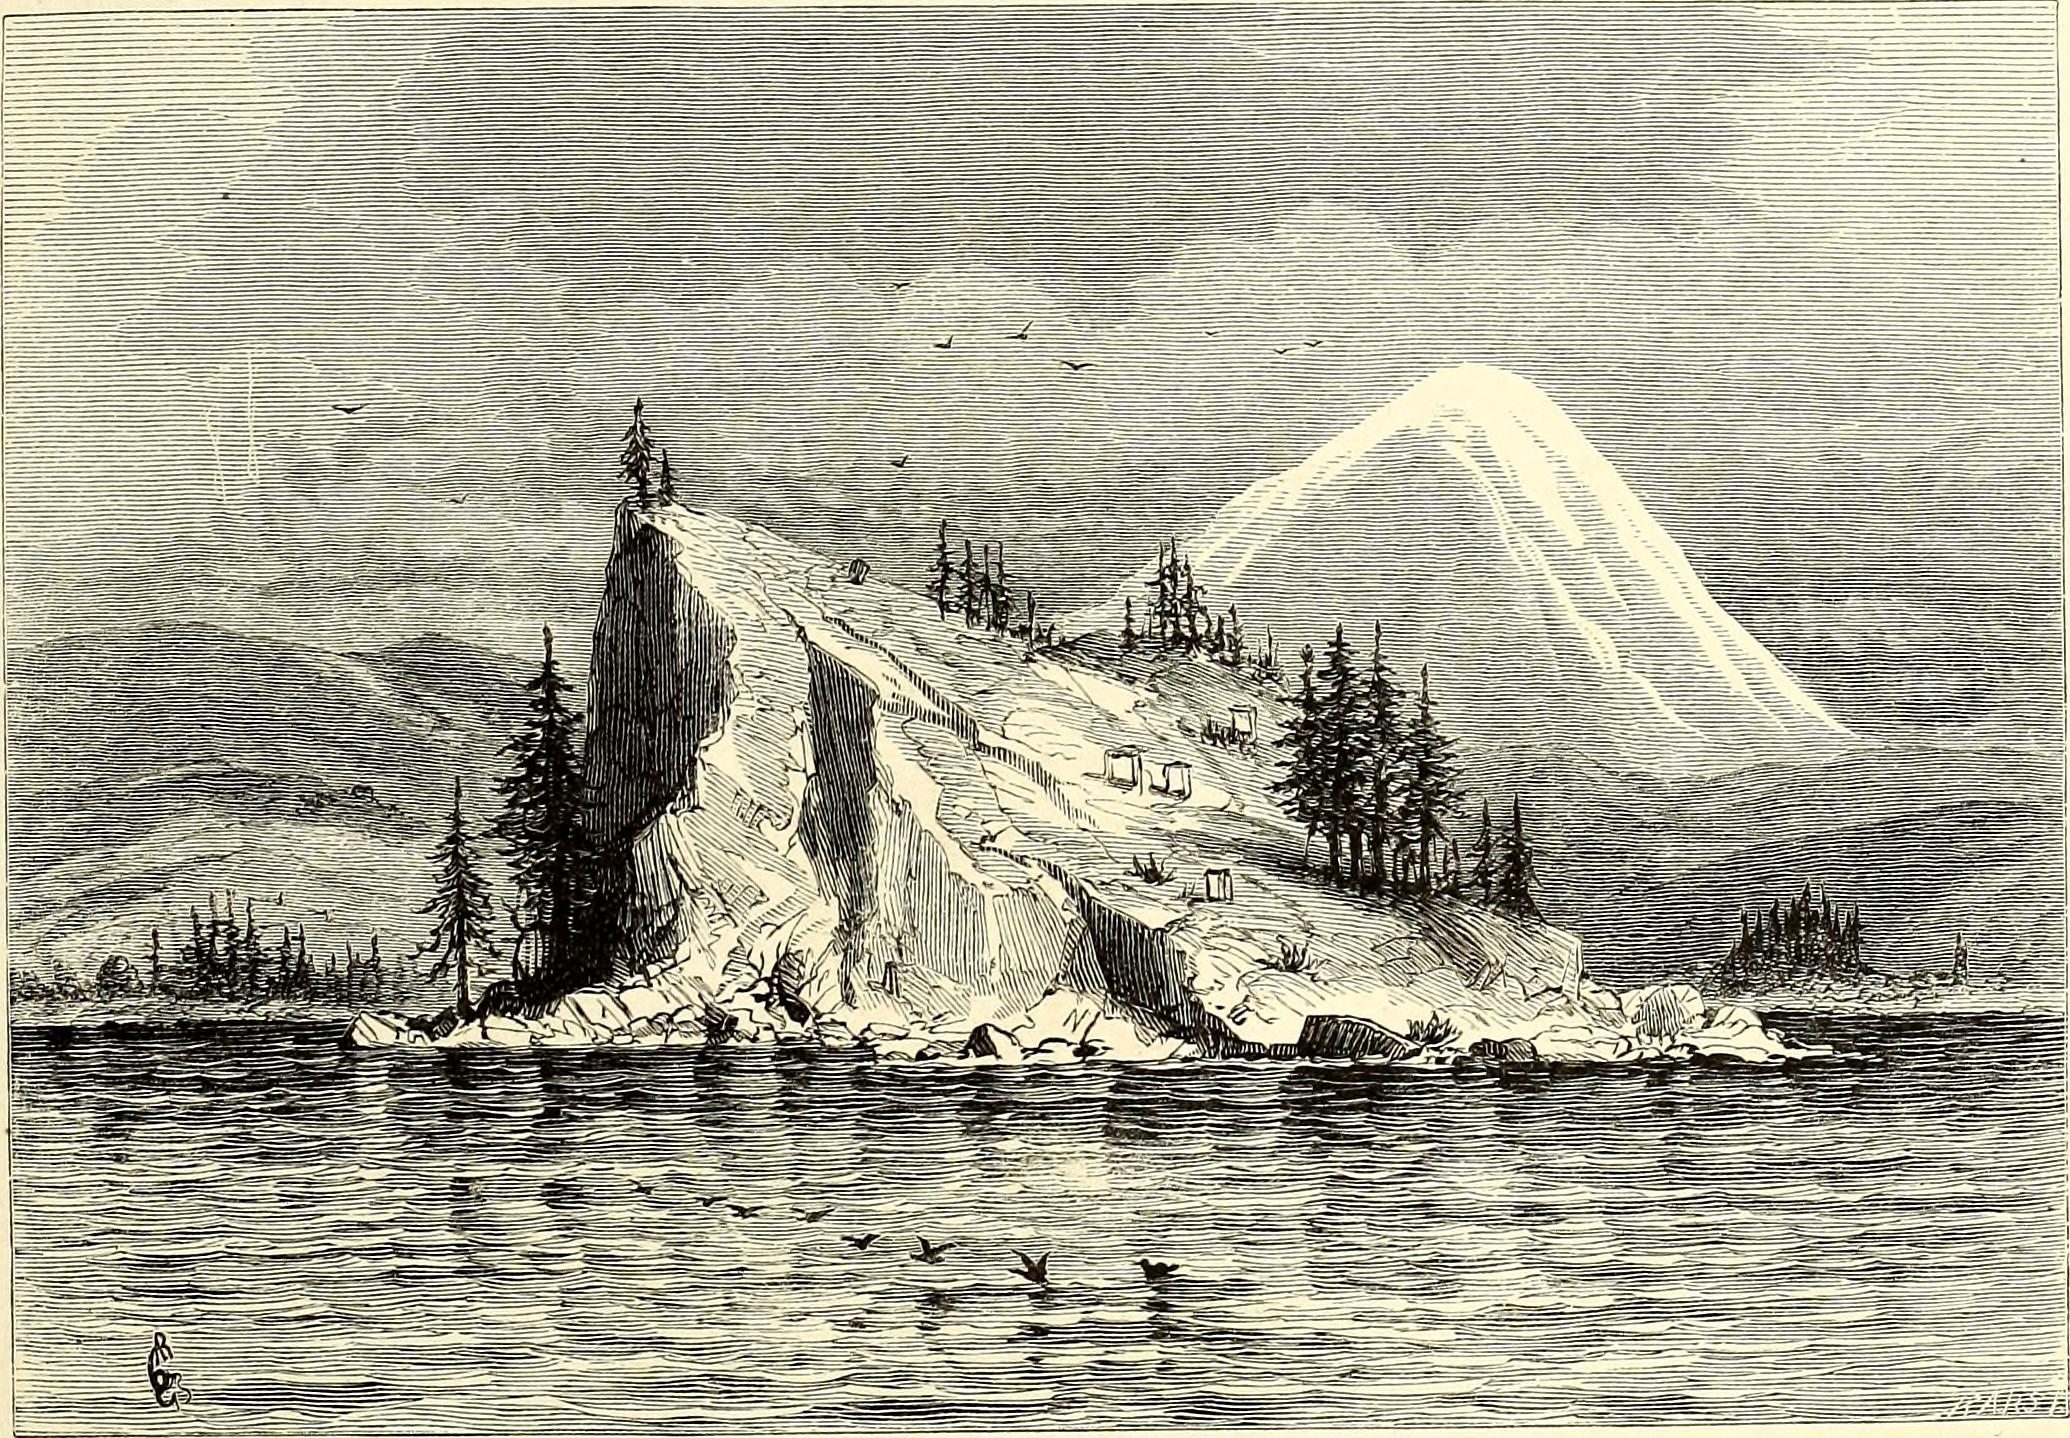
\includegraphics[width=\textwidth]{cover}
\newpage
\tableofcontents
\listoftables
\newpage

\begin{multicols}{2}
  
\section{Introduction}

This is a setting zine and toolkit for a far-north biome.
This zine contains some basic overview of the setting elements and an example map. \\

Some broad ideas are sketched, while many details are left out.
Many ideas are brought up and not pursued.
This allows you to fine--tune the setting as you please.
You should develop the ideas your find interesting to shape a campaign that is fun and unique to you.

\subsection*{What are the Northern Reaches?}

The Northern Reaches are the name for a region close to the poles of your world, one which is dominated by snowy and icy biomes: taiga, polar seas, and icy wastes. \\

It was once the realm of a great kingdom centuries ago, but a sudden onset of cold and ice quickly extinguished this society.
Now, however, the ice is slowly receding, revealing long-lost treasures. \\

The recession of the cold has allowed some settlers to come in and reclaim some of the land, some to settle more permanently and others looking to plunder this lost land. \\

They are not the only life out in the Reaches; many well--adapted creatures live in the wilderness outside of the settled towns.
The Reaches provide many natural resources for trade: lumber, ore, fish, and furs, but the living is tough.

\subsection*{Where are the Northern Reaches?}

You may use this setting as a stand-alone location, or incorporate it into a larger campaign world you have established or will establish.
Use this setting in a cold polar region.

\subsection*{What Kind of World is the Northern Reaches In?}

Anything you like.
A fitting world away from the Reaches is a large empire that has demand for natural resources from trade with the settlers of the Reaches.
It may have magic, some technology, or both; you get to decide. \\

The Reaches will be presented in a concrete way; that is, in line with certain setting assumptions:

\begin{itemize}
\item The world has some magic. These powers are not accessible to common folks, but secluded wizards are known to exist.
\item There are monsters and danger outside of civilization. Venturing far from home is a perilous undertaking.
\item Many centuries of past civilizations have existed and fallen. Many of their riches still are hidden out of sight. 
\end{itemize}

You may choose different setting assumptions, and it may make sense to modify, exclude, or rearrange elements presented here.


\section{Systems for Play}

This setting is designed for adventuring, and should be played with an appropriate system for this goal.
Such a system might include:

\begin{itemize}
\item decisive combat
\item adventuring incentives
\item useful gear
\item slow advancement (if any predetermined advancement)
\end{itemize}

In short, an OSR system should do the job.
However, you may not be using an OSR system, or looking for an alternative.
In this case, use the following as either a conversion guide or a minimalist system:

\begin{itemize}
\item 1 Hit die requires two \emph{hits} to deplete, and vice versa. This converts HP and damage.
\item specify special abilities in a specific but diegetic way.
\item Specify any character or NPC stats out of 20 for roll--under mechanics.
\end{itemize}

Anything else should be left to situation--specific rulings by the Referee.

\subsection*{Optional Survival Mechanics}

Consider using the following mechanics for heat, travel, and weather. \\

Track Heat Points in the same way as health (hit dice or hits).
To calculate heat point loss, subtract the exposure modifier from your heat capacity every hour.
Being near a source of heat restores all lost heat points.
If all heat points are lost, lose health points at the same rate as heat points. \\

These rules are expanded in Section \ref{sec:weather-outdoor}.

\section{Basic Geographies of the Setting}

In the northern reaches of the world, there are four predominant geographical regions one may find: mountain ranges, taiga forest, polar seas, and the polar caps. \\

{\centering
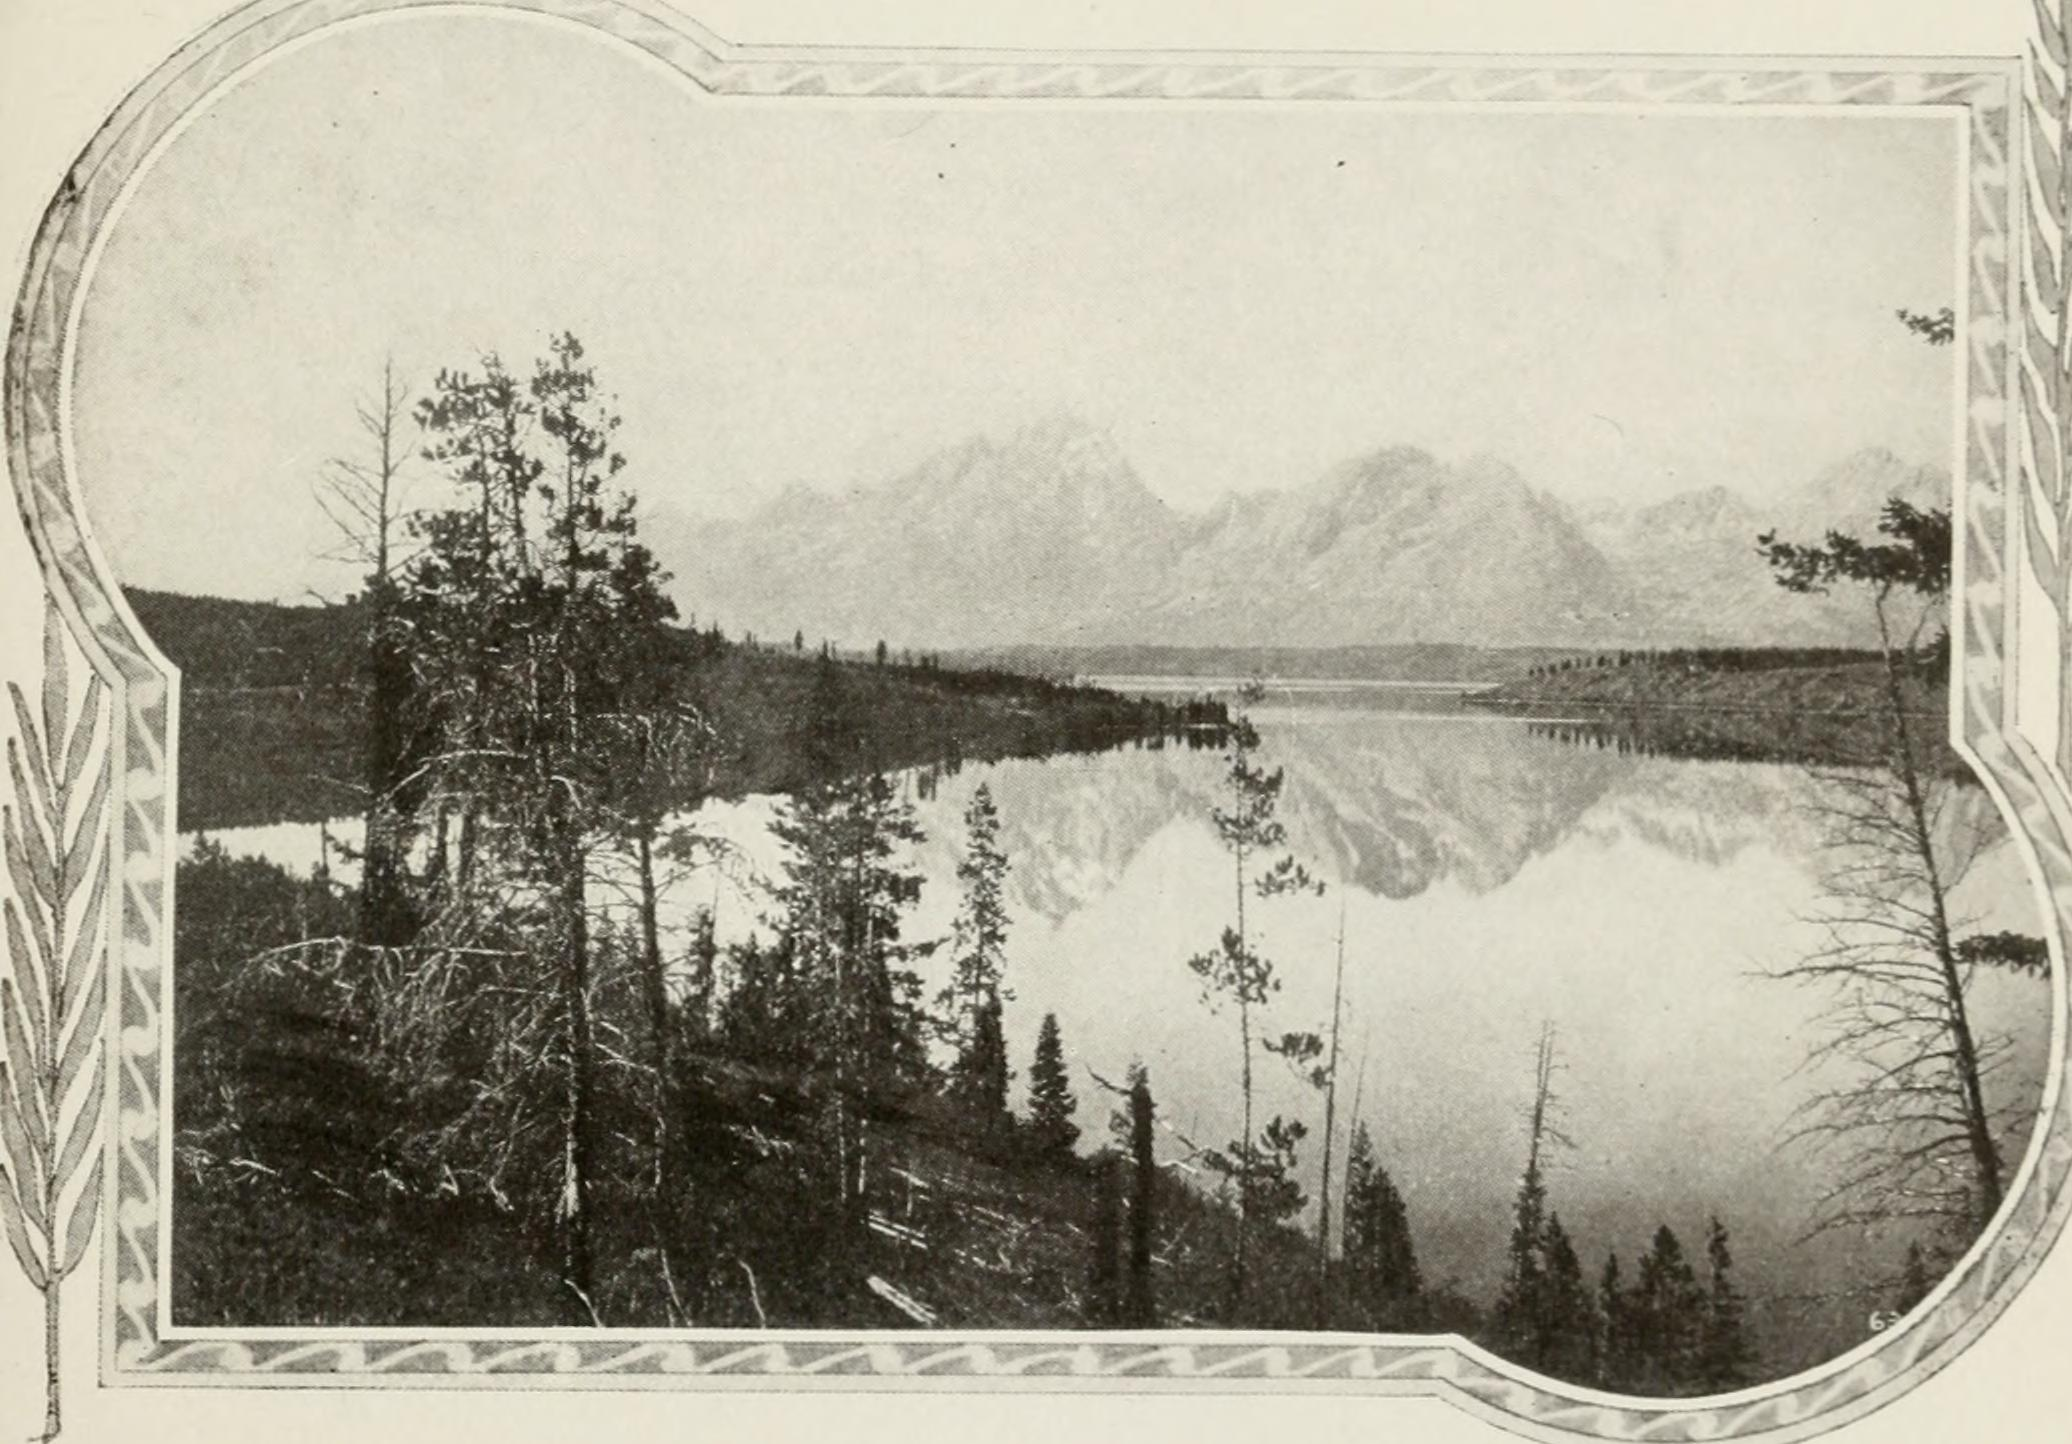
\includegraphics[width=\columnwidth]{geography-mountains}
}


\subsection*{Moutain Ranges}

Moutain ranges host a variety of life adjusted to the terrain and elevation. Small animals live amongst the many cracks and crevices, attracting bigger preadators. Verdant fields may span valleys between peaks, and caves in the mountains may stretch much deeper than at first glance. \\

Mountains are naturally a defensive geographical feature due to the difficult terrain. Transport through mountainous regions is slow and is often restricted to passes and paths. As a result, defensive human structures can be more common. \\

Consider the ecological and societal makeup in your montane regions.

\begin{itemize}
\item What larger monsters or beasts have come to pick off even the largest of mundane predators? How are they ajusted for a higher-altitude lifestyle?
\item What intelligent factions have taken up isolated residence among the peaks and valleys? Why have they decided to isolate themselves? How do they live in such an isolated environment?
\item What old structures remain in the mountains? Where do they lie among them?
\end{itemize}

Consider why a party of adventurous characters would visit such a place.

\begin{itemize}
\item Are there old ruins that might hide treasure or secrets?
\item Are there particular NPCs that have value to the party?
\item Are there rare biological ingredients here needed by the party?
\end{itemize}



\subsection*{Taiga Forest}

Northern forests see much snow, and as a result are full of moisture in spring. This can cause a variety of environmental conditions, from deep forests to wetlands and lakes. Natural resources are generally plentiful here, and human settlements are common. \\

Consider a specific region in your taiga region.

\begin{itemize}
\item What is the ecological makeup of this region? What are its main geographical features?
\item What kinds of peoples live here? What technology do they have, what is their relationship with their environment, and what relationships do they have with other nearby peoples?
\item What natural resources are unique to this region? What types of society flourish in an area with as mild of a climate?
\end{itemize}

\subsection*{Polar Seas}

Interspersed equally by icebergs and islands, the northern seas see more activity than one would expect, though not all is friendly. \\

Raiders will board the few trade ships around and ransack local villages. There are many fishers at work in the region, both near the shore and farther out, but weather, beast, and cold withhold plentiful bounties on every cast. \\

What activities are present in your northern seas?

\begin{itemize}
\item Who do raiders and marauders attack? What other societies are present?
\item How do player characters perform seafaring? Are they previously experienced, or do they need to hire a boat?
\item What sea creatures would interact with the party away from land?
\end{itemize}

\subsection*{Polar Caps}

There are no known standing structures beyond the northern seas. Only the coldest of winds blow. Snowy landscapes stretch interminably. Only the most foul of beasts live here.

\begin{itemize}
\item How have creatures adapted to the polar day and night cycles?
\item What preparation is needed to venture into this region? How long could one survive?
\item What treasure lies here? How can it be accessed?
\end{itemize}

\section{Weather and Cold}

{\centering 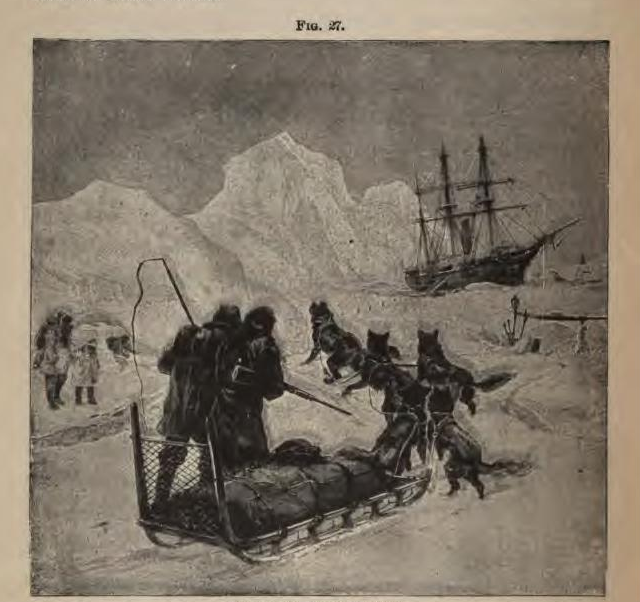
\includegraphics[width=\columnwidth]{arctic-sledders}
}

Retaining heat is of the utmost importance in all of the Reaches.
Some relevant system considerations have been mentioned already, and will be expanded here. \\

\subsection*{Weather Generation and Outdoor Survival}
\label{sec:weather-outdoor}

Weather is generated randomly for each period of 2 days. Roll d66 and consult Table \ref{tbl:weather}. The weather is generated for the local area for the period. \\

Players may consult locals for weather forecasts.
These forecasts have a chance of being wrong, consult Table \ref{tbl:weather}.
Weather for the next 4 days could be forecast, and should be rolled and played as per the roll, whether or not the forecast is accurate.
Player characters can forecast 1 day at a Commoner level within the first months of arriving, and better later on, depending on the adventuring done. \\

Warm clothing is essential for survival in most regions.
It increases heat capacity, which in turn allows more survival time without shelter.
To calculate full heat capacity, note what cold--weather clothing you have and use the max value of that many hit dice.
Consult Table \ref{tab:outdoor-survival} for heat capacity for various items of clothing. \\

If critically overexposed, you may apply conditions to the relevant characters.
For example, frostbite on exposed limbs. \\

Travel is slow or potentially impossible based on weather conditions.
To calculate travel time, use the current terrain type, recent conditions, and transportation type to modify the base rate of 12 miles/6 hours.
You may impose additional travel necessities situationally: Snow shoes may be necessary for heavily snowed areas, or horse travel may be impossible in mountainous regions. \\

At your discretion, you may apply cold weather mishaps to players.
Consult table \ref{tab:cold-events} for inspiration.
You may choose a mishap when a character runs out of heat points or due to in-game events.

\begin{table*}[t]
  \centering \large
  \begin{tabular}{| c || c || c ||}
    \hline
    & Snow (in/day) & Wind \\ \hline
    1 & 4 & Gusty \\
    2 & 2 & Gusty \\
    3 & 1 & Sustained Winds \\
    4 & 0 & Sustained Winds \\
    5 & -1 (melting) & Breezy \\
    6 & -2 (melting)  & Calm \\ \hline
  \end{tabular} \\

  \begin{tabular}{|c||c|}
    \hline Personage & Correct Forecast Chance (\%) \\ \hline
    Commoner  & 25 \% \\
    Explorer/Outdoorsman/Sailor & 50 \% \\
    Navigator & 75 \% \\ \hline
  \end{tabular}
  \caption{Weather Generation and Forecast Table}
  \label{tbl:weather}  
\end{table*}  


\begin{table*}[t]
  \centering \large
  \begin{tabular}{|c||c|}
    \hline Outdoor Conditions & Exposure Modifier \\ \hline
    Windy & +1 \\
    Gusty & +2 \\
    Light Precipitation & +1 \\
    Heavy Precipitation & +2 \\ \hline
  \end{tabular} \\

  \begin{tabular}{|c||c|}
    \hline Clothing Type & Heat Capacity \\ \hline
    Warm Coat & 2 HD \\
    Insulated Inner Layer & 4 HD \\
    Insulated Hats, Gloves, Socks, Boots, etc. & 2 HD \\
    Heavy Parka & 8 HD \\ \hline
  \end{tabular} \\

  \begin{tabular}{|p{0.2\textwidth}|l||p{0.2\textwidth}|l||p{0.1\textwidth}|l|}
    \hline Terrain Type & & Recent Weather & & Transportation Type & \\ \hline
    Road & +2 mi/6 hr & Clear& +0 & Walking & -2 mi/6 hr \\
    Mountain Path/Game Trail & +0 mi/6 hr & Light Snow & -2 mi/6 hr & Sled Dog & +6 mi/6 hr \\
    Overland/Wilderness & -2 mi/6 hr & Heavy Precipitation & -4 mi/6 hr & Skis & +4 mi/6 hr \\ \hline
  \end{tabular}
  \caption{Outdoor Survival Table}
  \label{tab:outdoor-survival}
\end{table*}

\begin{table*}[t]
  \centering
  \begin{tabular}{|c|c|}
    \hline Starts with... & Progresses to... \\ \hline
    Numbness & Frostbite \\
    Shivering & Hypothermia \\
    Itchiness & Trench foot \\
    Wet Layer & Compromised Clothing \\ 
    Loss of coordination & Dropped Item \\
    Chapped Skin & Open Wound \\ \hline
  \end{tabular}
  \caption{Cold Weather Events}
  \label{tab:cold-events}
\end{table*}


\section{Gear and Equipment}

Traveling through the reaches may require some specialized gear.
Consult Table \ref{tab:gear} for prices.

\begin{table*}[t]
  \centering
  \begin{tabular}{|r|l|} \hline
    Item & Cost (gold)  \\ \hline
    Coat & 10  \\
    Insulated Base Layer & 10 \\ 
    Hat/Gloves/Boots & 5 gold (total) \\
    Heavy Parka & 30 \\
    Toboggan Sled & 40 \\
    Skis & 30 \\
    Sled Dog Team (10 dogs and harness) & 120 \\
    Ice Axe & 20 \\
    Snow Shoes & 2 \\
 \hline \end{tabular}
  \caption{Cold-Weather Gear}
  \label{tab:gear}
\end{table*}

  \section{Factions and Peoples}

  Table \ref{tab:rumors} has rumors for the more well--known factions.
  You may choose which are true and which are false.

  \subsection*{Nomadic Raiders}

  Nomads who live by plundering and pillaging, occupying the shores before the empire moved in.
  Rather than being a unified force, this faction is highly decentralized, and can often clash internally.
  The various raiding groups are generally held together by a strong leader and a symbol.

  \begin{itemize}
  \item Haldr, the leader of the Eagles: this group prides itself on a wide view of its goals and aims. They are very strategic in their raids, and are excellent planners. If any group is the most well-known raiders of the empire, it is the Eagles.
  \item Arlir, the leader of the Bears: the most ferocious fighter in combat. They fight for glory and the sport of combat. They are especially brutal, channelling their idea of a bear's rage.
  \item Skete, leader of the Wolves: the most dogged in their pursuit. If a particular valuable is heard of, they will stop at nothing to track down and pursue its holder. Not as well--known.
  \end{itemize}

  Raiders are known to shun some magic, yet may hold practitioners of such in secret. These magics are predominantly divination and rituals for victory.

  When designing adventures around nomadic raiders, you may wish to consider:

  \begin{itemize}
  \item What powerful enemies have the Raiders angered in their usual raids?
  \item What highly-sought treasure has just been recovered?
  \item What areas of the Reaches are most vulnerable to attack?
  \end{itemize}

  \subsection*{The Orelian Church}

  The church of the empire is known for its dogmatic stance.
  In the Reaches, it fights to keep membership strong in order to tithe the locals and to convert any pre-existing native tribes. \\
  
  The church has a wide variety of assets to pull from.
  They have plenty of money, and their well-established position in the empire gives almost undue influence to the leaders of the small towns in the Reaches. \\

  The church is considered out of touch by non-adherents.
  As the church's focus is elsewhere on more lush lands, the doctrine can seem to allude to promises too outlandish or remote from the average settler's life.

  When designing conflicts of the Church, use the following as inspiration:

  \begin{itemize}
  \item What controversial action did the Church take recently?
  \item What local powers pull attention away from the Church's teachings?
  \item How much political power does the Church have in particular locations?
  \end{itemize}

  \subsection*{Ice Wizards}

  Scattered throughout the Reaches are the tops of free-standing towers peeking out from snow.
  Wizards live in these, completely self-sufficient.
  Most keep themselves warm and alive through ritual magic bonfires, by which they can grow food for themselves.
  Many have greenhouses within their towers, with many skylights.
  This maintains a delicate balance of heat, light, and nutrients for at most one person.
  Other self-sustainment mechanisms are possible, such as captive dragons. \\

  Answer the following when developing encounters around ice wizards:

  \begin{itemize}
  \item What useful asset might be held by this wizard?
  \item How has the wizard protected its abode from intruders?
  \item What is the wizard's stance towards outsiders?
  \end{itemize}

  \subsection*{Snow Dwarves}

  These are a mysterious and generally unknown people to the new settlers.
  Living far beneath mountain ranges, these architects' society is based on rapid consumption of natural resources.
  They are constantly digging for new building materials, new land to farm moss and fungi on, and precious metals for their scant trade with the surface world. \\

  Here are some hooks for characters to be introduced to Snow Dwarves:

  \begin{itemize}
  \item An exodus of dwarves to a small settler town due to uncovering a subterranean monster
  \item Dwarven miners are hiring surveyors and explorers for a recently discovered underground structure
  \item Dwarven farmers need retrieval of seeds from a vault under the earth.
  \end{itemize}

\begin{table*}[t]
  \centering
  \begin{tabular}{|p{0.25\textwidth}|}
    \hline Rumors of Raiders \\ \hline \hline
    If word of your treasure falls on the wrong ears, the wolves will hunt you down. \\ \hline
    The leader of the Eagles has a magic spyglass that can see any distance. \\ \hline
    They are the last survivors of the kingdom that existed before the ice covered all this. \\ \hline
    There is a group of shunned raiders, The Snakes, that are, literally, snake--people, cursed decades ago. \\ \hline
    If you see a longship on the waters, stay out of sight or flee. \\ \hline
    Most valuables raiders take end up at the bottom of the ocean. \\ \hline
  \end{tabular} \begin{tabular}{|p{0.25\textwidth}|}
                  \hline Rumors of the Orelian Church \\ \hline \hline
                  Those who speak against the Church publicly have been known to disappear. \\ \hline
                  The Church will offer bounty for reclaiming past holy sites. \\ \hline
                  The Archbishop of the Church can perform holy miracles. \\ \hline
                  The holy warriors serving the church have blessed weapons and spells. \\ \hline
                  The library of the Church houses very old historical texts. \\ \hline
                  Church priests do not allow idolatry within the settlements they have presence. \\ \hline
  \end{tabular} \begin{tabular}{|p{0.25\textwidth}|}
    \hline Rumors of Ice Wizards \\ \hline \hline
    Ice wizards will grant a spell to anyone providing food. \\ \hline
    They retreated into isolation because they were exiled for practicing black magic. \\ \hline
    Wizards keep vast libraries within their towers, you could find any piece of knowledge you seek. \\ \hline
    Ice wizards never leave their towers unless they are forced out. \\ \hline
    If you come across a stream of water under the snow, it might be coming from the warmth of a wizard tower. \\ \hline
    If you smell earth and soil in the permafrost, you can be sure you are near a wizard tower. \\ \hline
   \end{tabular}
   \caption{Faction Rumors}
  \label{tab:rumors}
\end{table*}


  \section{Adventures in the Reaches}

  Many pre-written modules can be reskinned for adventuring in the Reaches.
  Even taking a module without a far-north theme in mind can be made to fit by changing the names of monsters to Scandinavian folkloric names (e.g. zombies are now draugr).
  That said, some modules are aready perfect for the Reaches:

  \begin{itemize}
  \item \emph{Cavern of the Creeping Terror} by Kormar Publishing (for a sea-side hamlet)
  \item \emph{Falkrest Abbey} by Axian Spice (for an abandoned abbey in the mountains)
  \item \emph{Hel's Crow's Final Rest} by Ratking Productions (for a sea-side moral quandry)
  \item Any bits of \emph{Wolves Upon the Coast} by Luke Gearing
  \end{itemize}

  Other popular adventures may be adapted to the setting easily:

  \begin{itemize}
  \item \emph{The Black Wyrm of Brandonsford} by Chance Dudinack. Change the dragon to be called a Lindworm. Leads nicely into further interactions with dwarves.
  \item Many elements of \emph{Dolmenwood} by Gavin Norman can be used, e.g. the Abbey of St. Clewyd can have draugr instead of skeletons.
  \item \emph{Barrow of the Elf King} by Highland Paranormal Society has \'alfr in the tomb now.
  \end{itemize}

  \subsection*{Monsters in the Reaches}

  While you may pull from classic OSR bestiaries, consider giving the adventure flair based on Scandinavian mythology. Common threats could include Jotunn, trolls, n\"akki, or draugr, all of which you could find bestiary entries for as giants, trolls, nixies, and zombies. Kraken and Sea Serpents also fit nicely for nautical adventures. \\

  \subsection*{Sample Locales and Adventure}

  



\end{multicols}



\end{document}